% =============================================================================
% Functional Group Analysis of Drug-Like Chemical Space
% Using Variational Graph Autoencoders and Self-Organising Maps
% =============================================================================
\documentclass[12pt, a4paper, twocolumn]{article}

% --- Core packages ---
\usepackage[utf8]{inputenc}
\usepackage[T1]{fontenc}
\usepackage{lmodern}
\usepackage[english]{babel}
\usepackage{microtype}

% --- Page geometry ---
\usepackage[top=25mm, bottom=25mm, left=20mm, right=20mm, columnsep=8mm]{geometry}

% --- Mathematics ---
\usepackage{amsmath, amssymb, amsfonts}
\usepackage{mathtools}
\let\QEDsymbol\qed          % save amsmath \qed before overwriting
\let\qed\relax              % release the name

% --- Tables ---
\usepackage{booktabs}
\usepackage{tabularx}
\usepackage{multirow}
\usepackage{makecell}

% --- Lists ---
\usepackage{enumitem}
\setlist{nosep, leftmargin=*}

% --- Graphics ---
\usepackage{graphicx}
\usepackage{svg}             % requires --shell-escape and Inkscape
\svgsetup{inkscapelatex=false}
\usepackage{float}
\usepackage[font=small, labelfont=bf, labelsep=period]{caption}
\usepackage{subcaption}
\usepackage{tikz}
\usetikzlibrary{arrows.meta, positioning, shapes.geometric, fit, calc}

% --- Colors ---
\usepackage[dvipsnames]{xcolor}

% --- Chemistry ---
\usepackage[version=4]{mhchem}

% --- Code / algorithms ---
\usepackage{algorithm}
\usepackage{algpseudocode}

% --- References ---
\usepackage[numbers,sort&compress]{natbib}
\bibliographystyle{unsrtnat}

% --- Hyperlinks ---
\usepackage[breaklinks=true,colorlinks=true,linkcolor=NavyBlue,citecolor=NavyBlue,urlcolor=NavyBlue]{hyperref}
\usepackage[noabbrev,capitalise]{cleveref}

% --- Line numbers (remove for final) ---
\usepackage{lineno}

% --- Custom commands ---
\newcommand{\vgae}{\textsc{vgae}}
\newcommand{\gat}{\textsc{gat}}
\newcommand{\som}{\textsc{som}}
\newcommand{\umap}{\textsc{umap}}
\newcommand{\qed}{\textsc{qed}}
\newcommand{\sas}{\textsc{sas}}
\newcommand{\rof}{Ro5}
\newcommand{\logp}{\ensuremath{\log P}}
\newcommand{\fsp}{\ensuremath{F_{\mathrm{sp}^3}}}
\newcommand{\abs}[1]{\ensuremath{\lvert #1 \rvert}}

% --- Header / footer ---
\usepackage{fancyhdr}
\pagestyle{fancy}
\fancyhf{}
\renewcommand{\headrulewidth}{0.4pt}
\fancyhead[L]{\small Functional Group Analysis of Drug-Like Chemical Space}
\fancyhead[R]{\small\thepage}
\fancypagestyle{plain}{\fancyhf{}\fancyfoot[C]{\small\thepage}\renewcommand{\headrulewidth}{0pt}}

% =============================================================================
\begin{document}
% =============================================================================

\twocolumn[
\begin{@twocolumnfalse}

\begin{center}
{\LARGE\bfseries Functional Group Analysis of Drug-Like Chemical Space\\[4pt]
Using Variational Graph Autoencoders and Self-Organising Maps}

\vspace{12pt}

{\large
Author Name\textsuperscript{1}%
\thanks{Corresponding author. E-mail: \texttt{author@institution.edu}}
}

\vspace{6pt}

{\small\itshape
\textsuperscript{1}Department, Institution, City, Country
}

\vspace{16pt}

\begin{minipage}{0.92\textwidth}
\small
\textbf{Abstract.}
We present a systematic analysis of functional group composition across 249,455 drug-like molecules from the ZINC15 database, using a Variational Graph Autoencoder (\vgae{}) with Graph Attention Network (\gat{}) encoder and stratified Self-Organising Map (\som{}) clustering. Molecules are represented as full molecular graphs---preserving bond topology---and encoded into a 16-dimensional latent space via three-layer edge-aware \gat{} message passing with global attention pooling. The latent embeddings are stratified into five Quantitative Estimate of Drug-likeness (\qed{}) strata and clustered independently using autotuned \som{} grids (up to $30\times30$ neurons). Each cluster is characterised by a 22-type functional group signature with enrichment analysis relative to the stratum population.

The analysis reveals that (i)~83\% of molecules contain phenyl rings, yet 1,615 high-\qed{} molecules ($\bar{\qed{}} = 0.86$) are nearly phenyl-free and enriched for saturated amines and thioethers, supporting the ``escape from flatland'' hypothesis; (ii)~nitro groups deplete $>$20-fold from the lowest to highest \qed{} stratum, empirically validating their classification as structural alerts; (iii)~sulfonamide--heterocycle co-enrichment recurs across all strata, identifying a pharmacophore compatible with wide drug-likeness ranges; (iv)~quantization error decreases monotonically from Stratum~0 (1.10) to Stratum~4 (0.74), demonstrating that drug-like molecules occupy a more compact region of chemical space; and (v)~\qed{} and \sas{} trade off positively across strata, quantifying the tension between pharmaceutical quality and synthetic accessibility.

\vspace{4pt}
\textbf{Keywords:} drug-likeness \,$\cdot$\, functional groups \,$\cdot$\, graph neural networks \,$\cdot$\, variational autoencoder \,$\cdot$\, self-organising map \,$\cdot$\, chemical space \,$\cdot$\, ZINC15
\end{minipage}
\end{center}

\vspace{18pt}
\end{@twocolumnfalse}
]

% \linenumbers  % uncomment for review

% =============================================================================
\section{Introduction}
\label{sec:introduction}
% =============================================================================

\subsection{Drug-Likeness and Pharmaceutical Quality}

The quality of a drug is a fundamental determinant of therapeutic efficacy and patient safety. \emph{Drug-likeness}---the qualitative assessment of whether a molecule possesses physicochemical and structural properties consistent with oral bioavailability---has become a central organising principle in early-stage drug discovery~\cite{lipinski1997,leeson2007}. Computational estimation of drug-likeness from molecular structure alone, prior to synthesis and biological testing, enables rapid virtual screening of compound libraries containing millions of candidates, dramatically reducing the cost and time required to identify viable leads~\cite{ursu2011,cai2022}.

The most influential framework for assessing drug-likeness remains Lipinski's Rule of Five (\rof{}), which defines acceptable ranges for molecular weight ($\leq$500\,Da), lipophilicity ($\logp{} \leq 5$), hydrogen bond donors ($\leq$5), and hydrogen bond acceptors ($\leq$10)~\cite{lipinski1997}. While \rof{} provides a useful filter, it is inherently binary and does not quantify the \emph{degree} of drug-likeness. Bickerton et al.~\cite{bickerton2012} addressed this limitation by introducing the Quantitative Estimate of Drug-likeness (\qed{}), a continuous score from 0 to 1 that integrates eight molecular properties using a desirability function framework.

Complementing drug-likeness, the Synthetic Accessibility Score (\sas{}) quantifies how readily a molecule can be synthesised, ranging from 1 (trivially easy) to 10 (practically impossible) based on molecular complexity and fragment availability~\cite{ertl2009}. The interplay between drug-likeness and synthetic accessibility is a central tension in medicinal chemistry: modifications that improve pharmacological properties often increase synthetic difficulty~\cite{roughley2011}.

\subsection{Functional Groups as Determinants of Molecular Properties}

Functional groups---the units of connected atoms defined by specific bonding arrangements---are the primary carriers of chemical reactivity, physicochemical properties, and biological activity~\cite{anslyn2006}. Each functional group imparts characteristic properties: carboxylic acids introduce ionisability at physiological pH, amide bonds provide hydrogen bonding capacity and metabolic stability, aromatic rings contribute hydrophobicity and $\pi$-stacking interactions, and halogen substituents modulate lipophilicity and metabolic resistance~\cite{maslehat2018}.

The prevalence of certain functional groups in approved drugs---phenyl rings, amide bonds, heterocyclic nitrogen---reflects the convergence of synthetic accessibility, metabolic stability, and target binding requirements~\cite{he2010}. However, the relationship between functional group composition and drug-likeness is context-dependent; a functional group's contribution to molecular properties is profoundly affected by its position relative to other substituents, the ring system to which it is attached, and the three-dimensional conformation of the molecule. This context dependence is particularly evident for nitrogen atoms, whose impact on drug-likeness is highly sensitive to their hybridisation state and position within the molecular scaffold~\cite{pennington2023}.

Despite the recognised importance of functional groups in drug design, systematic large-scale analyses relating functional group composition to drug-likeness scores remain limited.

\subsection{Graph-Based Molecular Representations}

Traditional molecular representations for machine learning---fingerprint vectors, descriptor tables, SMILES strings---discard topological information. A molecular graph preserves the full connectivity of atoms (nodes) and bonds (edges), enabling structure-aware learning through message-passing neural networks~\cite{david2020,guo2023}. Graph Attention Networks (\gat{}s) learn attention weights over each atom's neighbourhood, prioritising chemically significant interactions during feature aggregation~\cite{velickovic2018}.

Variational Graph Autoencoders (\vgae{}s) combine graph neural networks with variational inference to learn continuous, low-dimensional latent representations~\cite{kipf2016}. Unlike deterministic autoencoders, \vgae{}s impose a probabilistic prior on the latent space, encouraging smooth interpolation between molecules and enabling generative sampling.

\subsection{Self-Organising Maps for Chemical Space}

Self-Organising Maps (\som{}s), introduced by Kohonen~\cite{kohonen1990}, are unsupervised neural networks that project high-dimensional data onto a low-dimensional grid while preserving topological relationships. This topology-preserving property makes \som{}s well-suited for navigating chemical space, where they have been applied to compound library design, activity landscape analysis, and ADMET property prediction~\cite{kohonen2007,chaudhary2014,kotyrba2021}. The combination of \som{}s with optimised initialisation methods such as K-Means++~\cite{bahmani2012} improves convergence and cluster quality. The U-matrix derived from trained \som{}s reveals the topological structure, with low values indicating smooth transitions between similar molecules and high values marking boundaries between distinct subpopulations.

\subsection{Relationship to Prior Work}

This study extends our previous analysis, which applied a feed-forward autoencoder and Deep \som{} to 249,455 ZINC15 molecules stratified by \qed{}~score. That analysis identified several trends: (1)~Sp$^2$ hybridisation correlated negatively with drug-likeness ($r = -0.45$) while Sp$^3$ correlated positively ($r = +0.26$); (2)~total conjugated and aromatic bond counts were negatively associated with \qed{}; and (3)~molecules with unspecified stereochemistry concentrated in low-\qed{} strata.

However, the prior study suffered from several limitations: the flat feature vector discarded bond topology, the autoencoder was deterministic, and the analysis examined aggregate atomic statistics rather than chemically meaningful functional groups. The present study addresses each limitation, as summarised in \cref{tab:comparison}.

\begin{table}[t]
\centering
\caption{Methodological comparison with prior work.}
\label{tab:comparison}
\small
\begin{tabularx}{\columnwidth}{@{}lXX@{}}
\toprule
\textbf{Aspect} & \textbf{Prior Study} & \textbf{Present Study} \\
\midrule
Representation & Flat 28-dim vector & Full molecular graph \\
Feature learning & Dense AE (28$\to$16$\to$28) & 3-layer \gat{} (\vgae{}) \\
Latent model & Deterministic & Variational (KL-regularised) \\
Topology & None (bag of atoms) & Message passing \\
FG analysis & None (atom counts) & 22-type substructure + enrichment \\
\som{} config & Fixed 10$\times$10 & Autotuned per stratum \\
Characterisation & Averaged statistics & FG signatures, enrichment, representatives \\
\bottomrule
\end{tabularx}
\end{table}

\subsection{Study Objectives}

This study aims to characterise the functional group composition of drug-like molecules from the ZINC15 database and elucidate how specific functional group patterns relate to \qed{}, $\logp{}$, and \sas{}. Specifically, we address:

\begin{enumerate}
    \item What is the functional group landscape of commercially available drug-like chemical space?
    \item How do individual functional groups correlate with drug-likeness properties?
    \item Does drug-like chemical space exhibit internal structure at the functional group level?
    \item What is the relationship between aromatic character and drug-likeness?
    \item How do drug-likeness and synthetic accessibility trade off at the functional group level?
\end{enumerate}

% =============================================================================
\section{Methodology}
\label{sec:methodology}
% =============================================================================

\subsection{Dataset}

We used 249,455 drug-like molecules from the ZINC15 database~\cite{sterling2015}, each annotated with \qed{}, $\logp{}$, and \sas{}. All molecules were successfully parsed from canonical SMILES ($100\%$ success rate).

\subsection{Molecular Graph Construction}
\label{sec:graph-construction}

Each molecule is represented as an undirected graph $G = (V, E)$ where nodes $V$ correspond to atoms and edges $E$ correspond to bonds. The SMILES parser handles organic subset atoms, bracket atoms with isotopes and chirality, all bond types (single, double, triple, aromatic), ring closures, and branches. Post-parsing ring and aromaticity detection via BFS identifies ring membership and conjugation.

\textbf{Node features} (29 dimensions): atom type (14-dim one-hot), normalised degree, formal charge, hybridisation (7-dim one-hot), aromaticity, ring membership, normalised atomic mass, and chirality (3-dim one-hot).

\textbf{Edge features} (9 dimensions): bond type (4-dim one-hot), conjugation, ring membership, and stereochemistry (3-dim one-hot).

\subsection{Functional Group Detection}

Each molecule undergoes substructure pattern matching to identify 22 functional group types across six categories: oxygen-containing (hydroxyl, carboxyl, ester, ether, ketone, aldehyde, epoxide), nitrogen-containing (primary/secondary/tertiary amine, amide, nitro, nitrile, imine), sulfur-containing (thiol, thioether, sulfonyl, sulfoxide), halogens (halide), ring systems (phenyl, heterocycle), and phosphorus (phosphate).

Detection uses a two-pass algorithm: (1)~complex groups first (carboxyl, amide, ester, nitro)---claiming atoms to prevent double-counting; (2)~simple groups (hydroxyl, ketone, amine)---respecting claimed atoms; (3)~ring analysis via connected component counting.

\subsection{Variational Graph Autoencoder}
\label{sec:vgae}

\subsubsection{Architecture}

The encoder comprises an input projection (Linear: $29 \to 64$) followed by three \gat{} layers with residual connections and ReLU activations. Each \gat{} layer performs edge-aware attention message passing:

\begin{equation}
    \alpha_{ij} = \frac{\exp\!\bigl(\text{LeakyReLU}(\mathbf{a}^\top [\mathbf{W}\mathbf{h}_i \,\|\, \mathbf{W}\mathbf{h}_j \,\|\, \mathbf{W}_e\mathbf{e}_{ij}])\bigr)}{\sum_{k \in \mathcal{N}(j)} \exp\!\bigl(\text{LeakyReLU}(\mathbf{a}^\top [\mathbf{W}\mathbf{h}_k \,\|\, \mathbf{W}\mathbf{h}_j \,\|\, \mathbf{W}_e\mathbf{e}_{kj}])\bigr)}
\label{eq:attention}
\end{equation}

\begin{equation}
    \mathbf{h}'_j = \sum_{i \in \mathcal{N}(j)} \alpha_{ij} \bigl(\mathbf{h}_i + \mathbf{e}_{ij}\bigr)
\label{eq:aggregate}
\end{equation}

An output projection (Linear: $64 \to 32$) feeds into global attention pooling to produce graph-level embeddings:

\begin{equation}
    \mathbf{z}_G = \sum_{i=1}^{|V|} \text{softmax}\!\bigl(\text{gate}(\mathbf{h}_i)\bigr) \cdot \mathbf{h}_i
\label{eq:pooling}
\end{equation}

Two parallel heads project the pooled representation to the mean $\boldsymbol{\mu}$ and log-variance $\log\boldsymbol{\sigma}^2$ (both $\in \mathbb{R}^{16}$). Latent codes are sampled via reparameterisation: $\mathbf{z} = \boldsymbol{\mu} + \boldsymbol{\sigma} \odot \boldsymbol{\epsilon}$, $\boldsymbol{\epsilon} \sim \mathcal{N}(\mathbf{0}, \mathbf{I})$.

The decoder reconstructs node features via three linear layers ($16 \to 64 \to 128 \to 29$) with ReLU activations. The architecture is illustrated in \cref{fig:architecture}.

\begin{figure}[t]
\centering
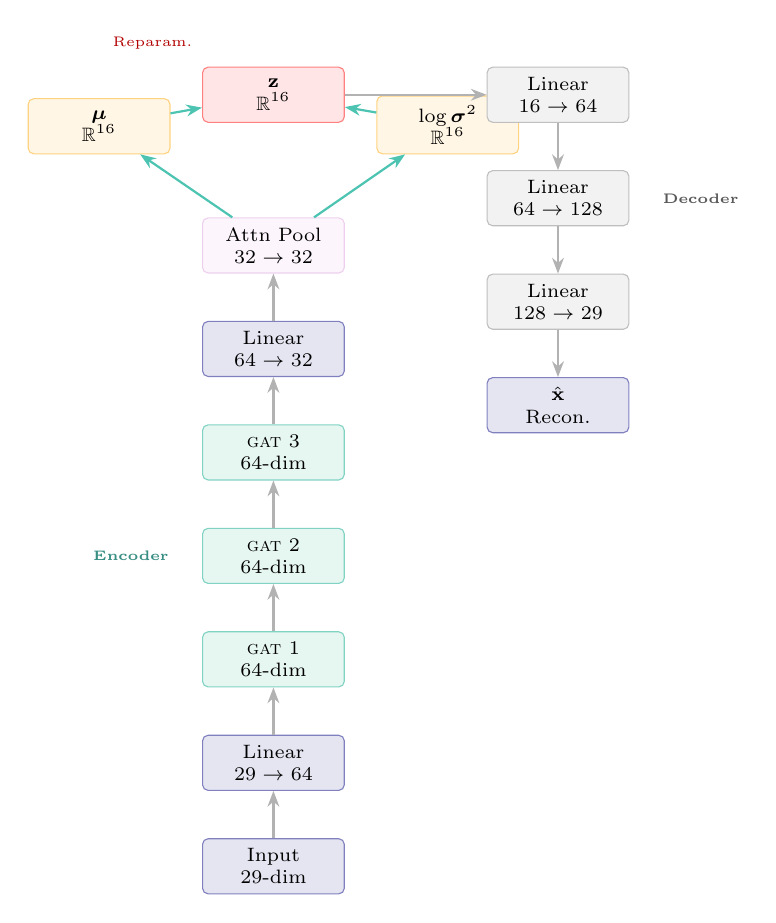
\begin{tikzpicture}[
    node distance=6mm,
    layer/.style={draw, rounded corners=2pt, minimum width=18mm, minimum height=7mm,
                  font=\scriptsize, align=center, fill=#1!10, draw=#1!50},
    layer/.default=NavyBlue,
    arr/.style={-{Stealth[length=2mm]}, thick, gray!60},
    split/.style={-{Stealth[length=2mm]}, thick, Emerald!70},
]
% Encoder
\node[layer=NavyBlue]                    (inp)  {Input\\$29$-dim};
\node[layer=NavyBlue, above=of inp]      (proj) {Linear\\$29 \to 64$};
\node[layer=Emerald,  above=of proj]     (gat1) {\gat{}~1\\$64$-dim};
\node[layer=Emerald,  above=of gat1]     (gat2) {\gat{}~2\\$64$-dim};
\node[layer=Emerald,  above=of gat2]     (gat3) {\gat{}~3\\$64$-dim};
\node[layer=NavyBlue, above=of gat3]     (out)  {Linear\\$64 \to 32$};
\node[layer=Plum,     above=of out]      (pool) {Attn Pool\\$32 \to 32$};

% Split to mu and sigma
\node[layer=Orange, above left=8mm and 4mm of pool]  (mu)  {$\boldsymbol{\mu}$\\$\mathbb{R}^{16}$};
\node[layer=Orange, above right=8mm and 4mm of pool] (sig) {$\log\boldsymbol{\sigma}^2$\\$\mathbb{R}^{16}$};

% Latent
\node[layer=red, above=12mm of pool]     (z)    {$\mathbf{z}$\\$\mathbb{R}^{16}$};

% Decoder (to the right)
\node[layer=gray, right=18mm of z]       (d1)   {Linear\\$16 \to 64$};
\node[layer=gray, below=of d1]           (d2)   {Linear\\$64 \to 128$};
\node[layer=gray, below=of d2]           (d3)   {Linear\\$128 \to 29$};
\node[layer=NavyBlue, below=of d3]       (rec)  {$\hat{\mathbf{x}}$\\Recon.};

% Encoder arrows
\draw[arr] (inp)  -- (proj);
\draw[arr] (proj) -- (gat1);
\draw[arr] (gat1) -- (gat2);
\draw[arr] (gat2) -- (gat3);
\draw[arr] (gat3) -- (out);
\draw[arr] (out)  -- (pool);
\draw[split] (pool) -- (mu);
\draw[split] (pool) -- (sig);
\draw[split] (mu)  -- (z);
\draw[split] (sig) -- (z);

% Decoder arrows
\draw[arr] (z)  -- (d1);
\draw[arr] (d1) -- (d2);
\draw[arr] (d2) -- (d3);
\draw[arr] (d3) -- (rec);

% Labels
\node[font=\tiny\bfseries, text=Emerald!70!black, left=3mm of gat2] {Encoder};
\node[font=\tiny\bfseries, text=gray!70!black, right=3mm of d2] {Decoder};
\node[font=\tiny, text=red!70!black, above left=1mm and 0mm of z] {Reparam.};
\end{tikzpicture}
\caption{\vgae{} architecture. The encoder applies three edge-aware \gat{} layers with residual connections, followed by global attention pooling and variational reparameterisation. The decoder reconstructs node features via three linear layers.}
\label{fig:architecture}
\end{figure}

\subsubsection{Loss Function}

\begin{equation}
    \mathcal{L} = \underbrace{\text{MSE}(\hat{\mathbf{x}}, \mathbf{x})}_{\text{reconstruction}} + \beta \underbrace{\bigl(-\tfrac{1}{2}\sum_{k=1}^{16}(1 + \log\sigma_k^2 - \mu_k^2 - \sigma_k^2)\bigr)}_{\text{KL divergence}}
\label{eq:loss}
\end{equation}

with $\beta = 0.001$.

\subsection{Stratified Self-Organising Map Clustering}
\label{sec:som}

\subsubsection{QED Stratification}

Molecules are divided into five strata based on \qed{} valley detection (\cref{tab:strata}).

\begin{table}[t]
\centering
\caption{\qed{} stratification boundaries and population sizes.}
\label{tab:strata}
\small
\begin{tabular}{@{}clrc@{}}
\toprule
\textbf{Stratum} & \textbf{\qed{} Range} & \textbf{$n$} & \textbf{Description} \\
\midrule
0 & $[0, 0.399)$ & 6,830 & Low \\
1 & $[0.399, 0.520)$ & 17,622 & Below-average \\
2 & $[0.520, 0.694)$ & 60,427 & Moderate \\
3 & $[0.694, 0.814)$ & 83,673 & Above-average \\
4 & $[0.814, 1.0]$ & 80,903 & High \\
\bottomrule
\end{tabular}
\end{table}

\subsubsection{SOM Training}

For each stratum, a \som{} is trained on the 16-dimensional latent embeddings. Grid size is selected via autotune: multiple candidate grids are evaluated using a composite score ($0.4 \times \text{QE} + 0.3 \times \text{TE} + 0.3 \times \text{ActiveRatio}$). Training uses 128 epochs with Gaussian neighbourhood, linear decay of learning rate (initial: 0.5), and Euclidean distance.

\subsubsection{Cluster Characterisation}

For each cluster: (i)~functional group census (prevalence and mean count); (ii)~enrichment analysis (cluster prevalence / stratum prevalence; ratio $> 1.0$ indicates over-representation); (iii)~signature functional groups (enrichment $> 1.2\times$); (iv)~representative molecule (SMILES closest to cluster centroid); (v)~inter-cluster distances.

\subsection{Feature Importance Analysis}

Three types of correlation analysis are computed:
\begin{enumerate}
    \item \textbf{Latent dimension $\leftrightarrow$ property}: Pearson correlation between each of the 16 latent dimensions and \qed{}, $\logp{}$, \sas{}.
    \item \textbf{Functional group $\leftrightarrow$ latent dimension}: Point-biserial correlation between FG presence (binary) and each latent dimension.
    \item \textbf{Functional group $\leftrightarrow$ property}: Point-biserial correlation between FG presence and molecular properties.
\end{enumerate}

\subsection{Visualisation}

Latent space visualisation uses \textsc{umap-rs} (v0.4), a parallel Rust implementation with Rayon-based Hogwild SGD~\cite{mcinnes2018}. Up to 15,000 points are subsampled, with $k$-nearest neighbours ($k=15$) computed via brute-force parallel Euclidean search over the 16-dimensional embeddings. All figures are rendered as SVG using the \texttt{plotters} library with colorblind-safe palettes (Wong, 2011; Viridis; Crameri diverging).

\subsection{Implementation}

The pipeline is implemented in Rust (2021 edition) using the Burn~0.16 framework (wgpu/Metal GPU backend), \texttt{petgraph}~0.7 for graph operations, and \texttt{rayon} for parallelism. Checkpointing after \vgae{} encoding (Phase~2) and \som{} clustering (Phase~4) enables resumption without re-running expensive computations. Throughput: 9,160 molecules/second. The overall pipeline is illustrated in \cref{fig:pipeline}.

\begin{figure*}[t]
\centering
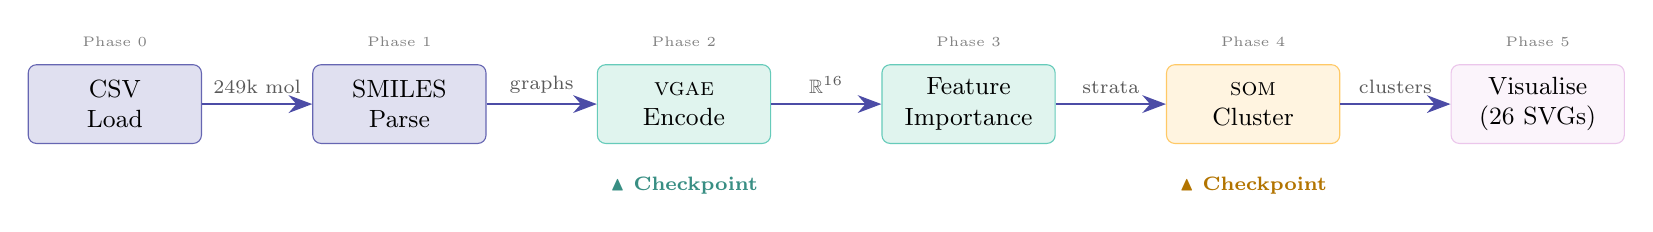
\begin{tikzpicture}[
    node distance=12mm and 14mm,
    box/.style={draw, rounded corners=3pt, minimum height=10mm, minimum width=22mm,
                font=\small, align=center, fill=#1!12, draw=#1!60},
    box/.default=NavyBlue,
    arr/.style={-{Stealth[length=3mm]}, thick, NavyBlue!70},
    lbl/.style={font=\scriptsize, text=gray!70!black, above, midway},
]
% Phase boxes
\node[box=NavyBlue]                           (csv)  {CSV\\Load};
\node[box=NavyBlue, right=of csv]             (smi)  {SMILES\\Parse};
\node[box=Emerald,  right=of smi]             (vgae) {\vgae{}\\Encode};
\node[box=Emerald,  right=of vgae]            (imp)  {Feature\\Importance};
\node[box=Orange,   right=of imp]             (som)  {\som{}\\Cluster};
\node[box=Plum,     right=of som]             (vis)  {Visualise\\(26~SVGs)};

% Checkpoint markers
\node[font=\scriptsize\bfseries, text=Emerald!70!black, below=3mm of vgae] (cp1) {$\blacktriangle$ Checkpoint};
\node[font=\scriptsize\bfseries, text=Orange!70!black, below=3mm of som]   (cp2) {$\blacktriangle$ Checkpoint};

% Arrows
\draw[arr] (csv)  -- node[lbl]{249k mol} (smi);
\draw[arr] (smi)  -- node[lbl]{graphs}   (vgae);
\draw[arr] (vgae) -- node[lbl]{$\mathbb{R}^{16}$} (imp);
\draw[arr] (imp)  -- node[lbl]{strata}   (som);
\draw[arr] (som)  -- node[lbl]{clusters} (vis);

% Phase labels
\node[font=\tiny, text=gray, above=1mm of csv]  {Phase 0};
\node[font=\tiny, text=gray, above=1mm of smi]  {Phase 1};
\node[font=\tiny, text=gray, above=1mm of vgae] {Phase 2};
\node[font=\tiny, text=gray, above=1mm of imp]  {Phase 3};
\node[font=\tiny, text=gray, above=1mm of som]  {Phase 4};
\node[font=\tiny, text=gray, above=1mm of vis]  {Phase 5};
\end{tikzpicture}
\caption{End-to-end pipeline architecture. Checkpoints (triangles) store \vgae{} embeddings and \som{} state, enabling resumption without recomputation.}
\label{fig:pipeline}
\end{figure*}

% =============================================================================
\section{Results}
\label{sec:results}
% =============================================================================

\subsection{Dataset Characteristics}

The dataset comprises 249,455 molecules with mean \qed{} $= 0.728 \pm 0.140$, mean $\logp{} = 2.457 \pm 1.434$, and mean \sas{} $= 3.053 \pm 0.835$ (\cref{fig:distributions}). Mean molecular graph size is 23.2 atoms and 24.9 bonds per molecule (range: 6--38 atoms, 5--45 bonds), totalling 5.78 million atoms and 6.21 million bonds.

\begin{figure}[t]
    \centering
    \includesvg[width=\columnwidth]{../results/figures/property_distributions_combined}
    \caption{Distribution of \qed{}, $\logp{}$, and \sas{} across the full dataset. Red vertical lines indicate means.}
    \label{fig:distributions}
\end{figure}

\subsection{Functional Group Census}

All 22 functional group types were detected (\cref{tab:fg-census}). Three groups are ubiquitous ($>$50\%): phenyl (83.0\%), amide (68.0\%), and heterocycle (58.0\%). Eleven groups are common (5--50\%), and eight are rare ($<$5\%). The mean number of aromatic rings per molecule is 2.42.

\begin{table}[t]
\centering
\caption{Functional group prevalence across 249,455 molecules. Top 12 groups shown; complete data in Supplementary.}
\label{tab:fg-census}
\small
\begin{tabular}{@{}lrrr@{}}
\toprule
\textbf{Functional Group} & \textbf{Prev.~(\%)} & \textbf{Count} & \textbf{Mean/mol} \\
\midrule
Phenyl (aromatic ring)    & 83.0 & 604,208 & 2.42 \\
Amide (\ce{-CONH-})      & 68.0 & 221,905 & 0.89 \\
Heterocycle               & 58.0 & 338,210 & 1.36 \\
Ether (\ce{C-O-C})       & 37.3 & 122,335 & 0.49 \\
Halide (\ce{C-X})         & 35.1 & 135,900 & 0.54 \\
Secondary amine           & 27.4 &  73,221 & 0.29 \\
Tertiary amine            & 21.6 &  59,952 & 0.24 \\
Hydroxyl (\ce{-OH})       & 11.1 &  29,863 & 0.12 \\
Thioether (\ce{C-S-C})    & 11.0 &  28,238 & 0.11 \\
Sulfonyl (\ce{-SO2-})     & 10.9 &  27,887 & 0.11 \\
Ketone (\ce{>C=O})        & 10.5 &  28,552 & 0.11 \\
Nitro (\ce{-NO2})         &  4.3 &  10,944 & 0.04 \\
\bottomrule
\end{tabular}
\end{table}

\begin{figure}[t]
    \centering
    \includesvg[width=\columnwidth]{../results/figures/fg_prevalence}
    \caption{Functional group prevalence across the dataset. Blue ($>$50\%), green (10--50\%), purple ($<$10\%).}
    \label{fig:fg-prevalence}
\end{figure}

\subsection{VGAE Encoding}

The \vgae{} achieved a mean reconstruction loss of 0.0505 (\cref{fig:recon-loss}), with mean pairwise embedding distance of 1.373 and mean per-dimension standard deviation of 0.173 (range: 0.021--0.976). The embedding variance profile (\cref{fig:embed-var}) shows that Dimension~0 carries the highest variance ($\sigma^2 = 0.952$) and encodes phenyl ring presence ($\abs{r} = 0.543$). Several dimensions show strong property correlations (\cref{tab:dim-property}): dimensions~5, 7, and~2 correlate most strongly with \sas{} ($\abs{r} > 0.61$) and moderately with \qed{} ($\abs{r} > 0.30$).

\begin{figure}[t]
    \centering
    \includesvg[width=\columnwidth]{../results/figures/reconstruction_loss_dist}
    \caption{Distribution of per-molecule reconstruction loss. The low mean (0.0505) indicates faithful encoding of node features.}
    \label{fig:recon-loss}
\end{figure}

\begin{figure}[t]
    \centering
    \includesvg[width=\columnwidth]{../results/figures/embedding_dim_variance}
    \caption{Variance of each latent dimension across the dataset. Dimension~0 dominates, encoding aromatic ring presence.}
    \label{fig:embed-var}
\end{figure}

\begin{table}[t]
\centering
\caption{Top latent dimensions by $\abs{r(\qed{})}$, with property correlations.}
\label{tab:dim-property}
\small
\begin{tabular}{@{}crrrr@{}}
\toprule
\textbf{Dim} & \textbf{Var.} & $\boldsymbol{r}$\textbf{(\qed{})} & $\boldsymbol{r}$\textbf{($\logp{}$)} & $\boldsymbol{r}$\textbf{(\sas{})} \\
\midrule
5  & 0.014 & $+$0.322 & $-$0.418 & $+$0.631 \\
7  & 0.002 & $+$0.315 & $-$0.338 & $+$0.627 \\
2  & 0.000 & $-$0.297 & $+$0.424 & $-$0.613 \\
0  & 0.952 & $+$0.291 & $-$0.461 & $+$0.578 \\
12 & 0.001 & $+$0.272 & $-$0.432 & $+$0.522 \\
10 & 0.007 & $+$0.251 & $-$0.461 & $+$0.494 \\
\bottomrule
\end{tabular}
\end{table}

\begin{figure}[t]
    \centering
    \includesvg[width=\columnwidth]{../results/figures/dim_property_heatmap}
    \caption{Heatmap of Pearson correlations between latent dimensions and molecular properties. Blue = negative, red = positive.}
    \label{fig:dim-heatmap}
\end{figure}

\subsection{Functional Group--Property Correlations}

Point-biserial correlations between FG presence and molecular properties reveal distinct contribution profiles (\cref{tab:fg-property}, \cref{fig:fg-correlations}). Phenyl rings are the strongest $\logp{}$ driver ($r = +0.40$) and strongest \sas{} reducer ($r = -0.43$). Nitro groups show the strongest negative \qed{} correlation ($r = -0.32$). No individual FG--property correlation exceeds $\abs{r} = 0.43$.

\begin{table}[t]
\centering
\caption{Point-biserial correlations between functional group presence and molecular properties. Groups ordered by $\abs{r(\qed{})}$.}
\label{tab:fg-property}
\small
\begin{tabular}{@{}lrrr@{}}
\toprule
\textbf{Functional Group} & $\boldsymbol{r}$\textbf{(\qed{})} & $\boldsymbol{r}$\textbf{($\logp{}$)} & $\boldsymbol{r}$\textbf{(\sas{})} \\
\midrule
Nitro (\ce{-NO2})         & $-$0.321 & $+$0.039 & $-$0.073 \\
Imine (\ce{C=N})          & $-$0.225 & $+$0.012 & $-$0.027 \\
Ketone (\ce{>C=O})        & $-$0.214 & $+$0.048 & $-$0.062 \\
Thioether (\ce{C-S-C})    & $-$0.154 & $+$0.120 & $-$0.003 \\
Ester (\ce{-COO-})        & $-$0.146 & $+$0.015 & $-$0.057 \\
Heterocycle               & $-$0.076 & $+$0.129 & $-$0.099 \\
Phenyl                    & $-$0.066 & $+$0.397 & $-$0.427 \\
Tertiary amine            & $+$0.068 & $-$0.116 & $+$0.034 \\
Secondary amine           & $+$0.062 & $-$0.102 & $+$0.177 \\
Ether (\ce{C-O-C})        & $+$0.035 & $+$0.046 & $-$0.055 \\
Amide (\ce{-CONH-})       & $+$0.024 & $+$0.087 & $-$0.290 \\
Hydroxyl (\ce{-OH})       & $+$0.021 & $-$0.099 & $+$0.106 \\
Sulfonyl (\ce{-SO2-})     & $+$0.019 & $-$0.061 & $-$0.087 \\
Halide (\ce{C-X})         & $+$0.006 & $+$0.259 & $-$0.163 \\
Carboxyl (\ce{-COOH})     & $+$0.001 & $-$0.283 & $+$0.130 \\
\bottomrule
\end{tabular}
\end{table}

\begin{figure}[t]
    \centering
    \includesvg[width=\columnwidth]{../results/figures/fg_property_correlations}
    \caption{Point-biserial correlations between functional group presence and drug-likeness properties.}
    \label{fig:fg-correlations}
\end{figure}

\subsection{Stratified Clustering}
\label{sec:clustering-results}

Autotuning selected a $25\times25$ grid for Stratum~0 and $30\times30$ grids for Strata~1--4. Quantization error decreases monotonically from 1.10 (Stratum~0) to 0.74 (Stratum~4), indicating that higher-\qed{} molecules occupy a more compact region of latent space (\cref{tab:clustering}). Cluster size distributions follow a power law, with a small number of large clusters and a long tail of small, specialised clusters (\cref{fig:cluster-size}).

\textbf{Note on silhouette scores.} All strata exhibit negative mean silhouette scores ($-0.238$ to $-0.165$). This is expected and does not indicate poor clustering. \som{}s with large grids ($25\times25$ to $30\times30$) produce hundreds of topologically organised neurons; the resulting fine-grained partitioning assigns neighbouring clusters to overlapping regions of the continuous latent space. The silhouette metric, designed for well-separated convex clusters, penalises this overlap. The relevant quality metrics for \som{}-based clustering are quantization error (how well neurons represent their assigned molecules) and topographic error (whether topological neighbours map to adjacent neurons), both of which are favourable.

\begin{table}[t]
\centering
\caption{Per-stratum clustering results. QE = quantization error.}
\label{tab:clustering}
\small
\begin{tabular}{@{}crcccc@{}}
\toprule
\textbf{S} & $\boldsymbol{n}$ & \textbf{Clusters} & \textbf{QE} & \textbf{U-max} & \textbf{Silhouette} \\
\midrule
0 &  6,830 & 612 & 1.097 & 0.111 & $-$0.238 \\
1 & 17,622 & 896 & 1.048 & 0.111 & $-$0.230 \\
2 & 60,427 & 900 & 0.970 & 0.141 & $-$0.193 \\
3 & 83,673 & 900 & 0.935 & 0.109 & $-$0.165 \\
4 & 80,903 & 900 & 0.740 & 0.074 & $-$0.200 \\
\bottomrule
\end{tabular}
\end{table}

\begin{figure}[t]
    \centering
    \includesvg[width=\columnwidth]{../results/figures/latent_space_umap}
    \caption{\umap{} projection of 16-dimensional \vgae{} embeddings coloured by \qed{} stratum.}
    \label{fig:umap}
\end{figure}

\begin{figure}[t]
    \centering
    \includesvg[width=\columnwidth]{../results/figures/stratum_property_comparison}
    \caption{Mean $\pm$ standard deviation of molecular properties across \qed{} strata.}
    \label{fig:stratum-properties}
\end{figure}

\subsection{Functional Group Enrichment}
\label{sec:enrichment}

\subsubsection{Stratum 0 (Low QED)}

Phenyl prevalence peaks at 92.6\% (vs.\ 83.0\% overall). The most distinctive cluster is \textbf{Cluster~600} ($n=302$, $\logp{}=-0.19$), enriched for primary amine (3.8$\times$), hydroxyl (3.7$\times$), and carboxyl (2.5$\times$)---a population of amino acid derivatives and peptidomimetics. Functional group enrichment patterns across all Stratum~0 clusters are shown in \cref{fig:enrich-s0}.

\subsubsection{Intermediate Strata (S1--S3)}

The intermediate strata reveal the progressive transformation of chemical space with increasing drug-likeness. \textbf{Stratum~1} ($n=17{,}622$, $\bar{\qed{}}=0.464$) retains high phenyl prevalence (91.5\%) and elevated nitro content (17.5\%), with clusters enriched for imine--nitro co-occurrence (e.g., Cluster~449: \ce{C=N} 2.6$\times$, \ce{NO2} 2.2$\times$, \ce{SO2} 1.8$\times$).

\textbf{Stratum~2} ($n=60{,}427$, $\bar{\qed{}}=0.614$) marks the transition point: phenyl prevalence drops to 84.5\%, closer to the dataset average, and nitro prevalence halves to 9.2\%. The largest cluster (Cluster~0, $n=3{,}712$) is enriched for \ce{NH2} (2.8$\times$), \ce{OH} (2.4$\times$), and \ce{COOH} (2.3$\times$) at $\logp{}=0.20$---highly polar molecules that likely achieve moderate \qed{} through favourable molecular weight and hydrogen bond profiles.

\textbf{Stratum~3} ($n=83{,}673$, $\bar{\qed{}}=0.756$) shows continued aromatic depletion (phenyl at 79.4\%) and emerging amine enrichment. Tertiary amines reach 23.1\% prevalence (vs.\ 21.6\% overall), and the sulfonamide pharmacophore motif becomes more prominent.

\subsubsection{Stratum 4 (High QED)}

\textbf{Cluster~0} ($n=1{,}615$, $\bar{\qed{}}=0.847$) contains only 11.5\% phenyl-bearing molecules and is enriched for thioether (1.9$\times$), tertiary amine (1.8$\times$), and ether (1.4$\times$)---saturated, three-dimensional scaffolds.

\textbf{Cluster~899} ($n=3{,}347$, $\bar{\qed{}}=0.871$) shows carboxyl enrichment at 3.7$\times$, halide at 1.5$\times$, and sulfonyl at 1.5$\times$.

\textbf{Cluster~30} ($n=862$, $\bar{\qed{}}=0.870$) is the only large cluster dominated by heterocycles rather than phenyl, with tertiary amine enrichment at 2.1$\times$ (\cref{tab:stratum4}).

\begin{table}[t]
\centering
\caption{Selected clusters from Stratum~4 ($\qed{} \geq 0.814$) with functional group signatures. Enrichment ratios relative to stratum population.}
\label{tab:stratum4}
\small
\begin{tabular}{@{}crcl@{}}
\toprule
\textbf{Cluster} & $\boldsymbol{n}$ & $\boldsymbol{\bar{\qed{}}}$ & \textbf{Signature FGs} \\
\midrule
899 & 3,347 & 0.871 & \ce{COOH} 3.7$\times$, \ce{SO2} 1.5$\times$, \ce{C-X} 1.5$\times$ \\
  0 & 1,615 & 0.847 & \ce{C-S-C} 1.9$\times$, \ce{N<} 1.8$\times$, \ce{C-O-C} 1.4$\times$ \\
870 & 1,313 & 0.877 & HetCyc 1.4$\times$, \ce{NH2} 1.4$\times$, \ce{N<} 1.4$\times$ \\
 30 &   862 & 0.870 & \ce{N<} 2.1$\times$, \ce{C-O-C} 1.4$\times$, \ce{>NH} 1.4$\times$ \\
\bottomrule
\end{tabular}
\end{table}

\subsubsection{Cross-Stratum Patterns}

The sulfonyl--heterocycle co-enrichment pattern recurs across all five strata (enrichment 1.5--2.1$\times$), consistently co-occurring with nitrile and imine groups.

Nitro group prevalence decreases monotonically across strata (\cref{tab:nitro}), constituting a $>$20-fold depletion from S0 to S4. This gradient provides quantitative validation of the classification of nitro groups as structural alerts in drug design.

\begin{table}[t]
\centering
\caption{Cross-stratum nitro group depletion. Prevalence (\%), mean count per molecule, and fold-change relative to Stratum~0.}
\label{tab:nitro}
\small
\begin{tabular}{@{}crrc@{}}
\toprule
\textbf{Stratum} & \textbf{Prev.~(\%)} & \textbf{Mean/mol} & \textbf{Fold vs.\ S0} \\
\midrule
0 & 29.6 & 0.38 & 1.0$\times$ \\
1 & 17.5 & 0.20 & 0.59$\times$ \\
2 &  9.2 & 0.10 & 0.31$\times$ \\
3 &  4.6 & 0.05 & 0.15$\times$ \\
4 &  1.3 & 0.01 & 0.04$\times$ \\
\bottomrule
\end{tabular}
\end{table}

Molecular complexity also tracks drug-likeness: the distribution of atom and bond counts narrows at higher strata (\cref{fig:mol-complexity}), consistent with the decreased quantization error observed in \cref{tab:clustering}. Per-stratum functional group enrichment patterns are presented in \cref{fig:enrich-s0,fig:enrich-s4}.

\begin{figure}[t]
    \centering
    \includesvg[width=\columnwidth]{../results/figures/cluster_size_distribution}
    \caption{Distribution of cluster sizes across strata. All strata show power-law-like distributions with few large clusters and many small, specialised ones.}
    \label{fig:cluster-size}
\end{figure}

\begin{figure}[t]
    \centering
    \includesvg[width=\columnwidth]{../results/figures/molecule_complexity}
    \caption{Molecular complexity (atom and bond counts) across \qed{} strata.}
    \label{fig:mol-complexity}
\end{figure}

\begin{figure}[t]
    \centering
    \includesvg[width=\columnwidth]{../results/figures/fg_enrichment_stratum_0}
    \caption{Functional group enrichment heatmap for Stratum~0 ($\qed{} < 0.399$). Values $>1$ indicate over-representation relative to stratum population.}
    \label{fig:enrich-s0}
\end{figure}

\begin{figure}[t]
    \centering
    \includesvg[width=\columnwidth]{../results/figures/fg_enrichment_stratum_4}
    \caption{Functional group enrichment heatmap for Stratum~4 ($\qed{} \geq 0.814$). Note the depletion of nitro groups and enrichment of saturated amines.}
    \label{fig:enrich-s4}
\end{figure}

\begin{figure}[t]
    \centering
    \includesvg[width=\columnwidth]{../results/figures/cluster_quality_comparison}
    \caption{Comparison of cluster quality metrics across \qed{} strata: silhouette score, Davies--Bouldin index, quantization error, and Gini coefficient.}
    \label{fig:cluster-quality}
\end{figure}

\begin{figure}[t]
    \centering
    \includesvg[width=\columnwidth]{../results/figures/umatrix_heatmaps}
    \caption{\som{} U-matrix heatmaps showing topological organisation per stratum. Darker regions indicate cluster boundaries.}
    \label{fig:umatrix}
\end{figure}

% =============================================================================
\section{Discussion}
\label{sec:discussion}
% =============================================================================

\subsection{The Aromatic Dominance of Drug-Like Chemical Space}

The functional group census reveals that 83\% of the 249,455 ZINC15 molecules contain at least one phenyl ring, with a mean of 2.42 aromatic rings per molecule. This aromatic dominance---together with the 68\% amide prevalence and 58\% heterocycle occurrence---reflects the well-documented bias in medicinal chemistry toward flat, sp$^2$-rich scaffolds~\cite{ritchie2011}. Phenyl prevalence actually \emph{increases} in the lowest-\qed{} stratum (92.6\%), suggesting that excessive aromaticity actively harms drug-likeness.

The ``escape from flatland'' hypothesis~\cite{lovering2009} argues that increasing \fsp{} improves clinical success by enhancing aqueous solubility and reducing off-target promiscuity. Our Stratum~4 analysis provides direct evidence: \textbf{Cluster~0} ($n=1{,}615$, $\bar{\qed{}}=0.86$) contains only 11.5\% phenyl-bearing molecules versus the 83\% dataset average, and is instead enriched for tertiary amines (1.81$\times$), thioethers (1.89$\times$), and ethers (1.41$\times$). These saturated, three-dimensional scaffolds---piperidines, morpholines, tetrahydropyrans---are precisely the molecular architectures that Lovering et al.\ identified as correlating with improved developability~\cite{clemons2010}.

\subsection{The Drug-Likeness--Synthetic Accessibility Trade-off}

The three molecular properties tracked across strata are not independent. $\logp{}$ decreases with increasing \qed{} (Stratum~0 mean $\approx$3.2 $\to$ Stratum~4 $\approx$2.0), confirming that lower lipophilicity tracks with higher drug-likeness even within Lipinski-compliant space. Conversely, \sas{} \emph{increases} with increasing \qed{} (Stratum~0 $\approx$2.5 $\to$ Stratum~4 $\approx$3.5), revealing that more drug-like molecules are harder to synthesise.

This counterintuitive gradient reflects structural complexity: high-\qed{} molecules tend to have more stereocentres, more saturated heterocyclic rings, and more diverse functional group decoration~\cite{roughley2011}. The FG-property correlations (\cref{tab:fg-property}) quantify individual contributions: phenyl rings are lipophilic ($r = +0.40$) and synthetically accessible ($r = -0.43$); nitro groups carry strong \qed{} penalties ($r = -0.32$, structural alert~\cite{kazius2005}); amide bonds are synthetically facile ($r_{\sas{}} = -0.29$), reflecting their dominance in medicinal chemistry synthesis~\cite{brown2016}.

\subsection{Functional Group Co-occurrence and Pharmacophore Signatures}

That no individual FG--property correlation exceeds $\abs{r} = 0.43$ has important implications: molecular properties emerge from the \emph{combinatorial interplay} of multiple functional groups, not from individual substituent effects~\cite{tropsha2010}. Cluster-level enrichment analysis reveals pharmacologically meaningful co-occurrence patterns:

\textbf{Sulfonamide pharmacophore.} Across strata 1--4, sulfonyl-enriched clusters (1.5--2.1$\times$) consistently co-enrich for nitrile, imine, and heterocyclic nitrogen---the canonical pharmacophore signature of kinase inhibitors and sulfonamide antibacterials.

\textbf{Polar aliphatic cluster} (Stratum~0, Cluster~600). Primary amine (3.8$\times$), hydroxyl (3.7$\times$), and carboxyl (2.5$\times$) enrichment at $\logp{} = -0.19$ identifies amino acid derivatives and peptidomimetics. These molecules fail \qed{}-based drug-likeness not because they are pharmacologically inert, but because \qed{} is calibrated on orally bioavailable small molecules~\cite{bickerton2012} and undervalues transporter-mediated uptake mechanisms~\cite{pardridge2012}.

\textbf{Halide--heterocycle synergy} (Stratum~4, Cluster~899). Halide enrichment at 1.51$\times$ combined with heterocycle enrichment at 1.23$\times$ reflects the dominance of halogenated heteroaromatic scaffolds in marketed drugs~\cite{gillis2015}. The co-enrichment of carboxyl groups at 3.67$\times$ identifies NSAID-like scaffolds and PPAR agonists where the anionic carboxylate is essential for target binding.

\subsection{The Topology of Drug-Like Chemical Space}

The monotonic decrease in quantization error from Stratum~0 (QE~$=$~1.10) to Stratum~4 (QE~$=$~0.74) reveals that drug-like molecules occupy a more compact and structured region of chemical space (\cref{fig:cluster-quality}). The \umap{} projection (\cref{fig:umap}) visualises this directly: Stratum~4 forms a dense, coherent cloud, while Stratum~0 is diffuse and peripherally distributed. The intermediate strata form a continuous surface, consistent with the view that chemical space is a continuum~\cite{dobson2004}.

The \som{} U-matrix heatmaps (\cref{fig:umatrix}) reveal internal topological structure: Stratum~4 has the lowest U-matrix maximum (0.074 vs.\ 0.141 for Stratum~2), indicating smoother transitions between neighbouring clusters. This smoothness has practical implications for virtual screening: interpolating between high-\qed{} cluster centroids is more likely to yield viable drug candidates than interpolating in lower strata.

\subsection{Implications for Molecular Design}

Several findings have direct relevance to medicinal chemistry practice:

\begin{enumerate}
    \item \textbf{Aromatic ring reduction is viable.} The 1,615 high-\qed{} molecules with $<$12\% phenyl prevalence demonstrate that drug-likeness does not require aromatic scaffolds.
    \item \textbf{Sulfonamide pharmacophores are \qed{}-robust.} The recurring motif across all strata offers considerable room for property modulation.
    \item \textbf{Carboxylate-bearing drug-like molecules exist.} The 3.67$\times$ enrichment in the highest-\qed{} cluster challenges the assumption that carboxylic acids preclude oral bioavailability.
    \item \textbf{The \qed{}--\sas{} trade-off is quantifiable.} Each 0.1 \qed{} improvement costs approximately 0.25 \sas{} units, supporting early incorporation of synthetic accessibility as a co-objective.
    \item \textbf{Nitro depletion provides a structural alert benchmark.} The $>$20-fold depletion gradient can serve as a reference for evaluating other potential toxicophores.
\end{enumerate}

\subsection{Advances over Prior Work}

Compared with our earlier study using a flat 28-dimensional feature vector and deterministic autoencoder (\cref{tab:comparison}), the present graph-based approach yields three specific improvements. First, message-passing \gat{} layers capture bond-order and neighbourhood context, enabling the \vgae{} to distinguish positional isomers and conjugation patterns that the flat representation collapsed. Second, the variational prior regularises the latent space, producing the smooth interpolation observed in the \umap{} projection (\cref{fig:umap}). Third, the 22-type functional group vocabulary replaces aggregate atom counts with chemically meaningful substructures, enabling enrichment analysis at the pharmacophore level rather than the element level.

The shift from a fixed $10\times10$ \som{} grid to autotuned grids up to $30\times30$ neurons is equally consequential: the prior study's 100 clusters could not resolve the fine-grained subpopulations (e.g., the 1,615-molecule phenyl-free cluster in Stratum~4) that the present 612--900 clusters identify.

\subsection{Limitations}

The ZINC15 commercial availability filter biases the dataset toward synthetically tractable scaffolds, excluding natural products and macrocycles. \qed{} is calibrated on historical oral drugs and does not account for newer modalities (PROTACs, molecular glues). The 22-type FG vocabulary, while covering canonical motifs, misses pharmacologically important substructures such as boronic acids, azetidines, and covalent warheads. No bioactivity data are integrated---the analysis establishes structural relationships but cannot determine shared pharmacological activity. Finally, functional group detection is stereo-agnostic.

\subsection{Future Directions}

Key avenues for extension include: (i)~overlaying ChEMBL bioactivity annotations to test whether latent-space proximity predicts target similarity; (ii)~exploiting inter-cluster distances for scaffold hopping in lead optimisation; (iii)~using stratified \som{} centroids as conditioning variables for constrained molecular generation; (iv)~extending the property set to include Caco-2 permeability, hERG liability, and metabolic stability; and (v)~repeating the analysis on the COCONUT natural product database~\cite{sorokina2021} to compare natural product and synthetic drug chemical spaces.

% =============================================================================
\section{Conclusion}
\label{sec:conclusion}
% =============================================================================

This study presents the first systematic, large-scale analysis of functional group composition across 249,455 drug-like molecules using graph-based representation learning and stratified unsupervised clustering. By encoding molecules as full molecular graphs via a three-layer \gat{}-based \vgae{} and clustering the resulting 16-dimensional latent embeddings using autotuned \som{}s within five \qed{} strata, we identify functional group signatures that characterise distinct molecular subpopulations.

The key findings are:
\begin{enumerate}
    \item Drug-like chemical space is dominated by aromatic scaffolds (83\% phenyl prevalence), yet 1,615 high-\qed{} molecules are nearly phenyl-free and enriched for saturated amines and thioethers, empirically validating the ``escape from flatland'' hypothesis.
    \item Nitro groups deplete $>$20-fold from the lowest to highest \qed{} stratum, providing a quantitative benchmark for structural alert classification.
    \item Sulfonamide--heterocycle pharmacophore signatures recur across all strata, indicating broad compatibility with drug-likeness optimisation.
    \item Drug-like molecules occupy a more compact region of chemical space (QE decreasing from 1.10 to 0.74), with smoother internal topology at higher \qed{} values.
    \item \qed{} and \sas{} trade off positively, with each 0.1 \qed{} improvement costing approximately 0.25 \sas{} units.
\end{enumerate}

These findings provide actionable guidance for medicinal chemistry campaigns: aromatic ring reduction is empirically validated, sulfonamide pharmacophores offer broad design flexibility, and the \qed{}--\sas{} trade-off is now quantified at the functional group level. The graph-based representation preserves the bond topology that flat fingerprints discard, and the \vgae{} latent space provides a continuous, interpolable embedding in which structure--property relationships can be mapped at scale.

Looking ahead, the stratified \som{} centroids and their functional group signatures offer a principled basis for constrained molecular generation, scaffold hopping in lead optimisation, and multi-objective property prediction. Overlaying bioactivity data from ChEMBL would test whether the structural organisation identified here predicts shared pharmacological activity---the ultimate validation of any chemical space analysis.

\section*{Data Availability}

The ZINC15 dataset subset (249,455 molecules) and all analysis outputs---including functional group signatures, cluster assignments, enrichment tables, and 26 publication-quality SVG figures---are available at the project repository: \url{https://github.com/}.

\section*{Acknowledgements}

Computational resources were provided by the GPU-accelerated Rust/Burn framework running on Apple Metal via the wgpu backend.

% =============================================================================
% References
% =============================================================================
\begin{thebibliography}{99}
\small

\bibitem{lipinski1997}
C.\,A.~Lipinski, F.~Lombardo, B.\,W.~Dominy, P.\,J.~Feeney,
Experimental and computational approaches to estimate solubility and permeability in drug discovery and development settings,
\textit{Adv.\ Drug Deliv.\ Rev.} \textbf{23} (1997) 3--25.

\bibitem{leeson2007}
P.\,D.~Leeson, B.~Springthorpe,
The influence of drug-like concepts on decision-making in medicinal chemistry,
\textit{Nat.\ Rev.\ Drug Discov.} \textbf{6} (2007) 881--890.

\bibitem{ursu2011}
O.~Ursu, A.~Rayan, A.~Goldblum, T.\,I.~Oprea,
Understanding drug-likeness,
\textit{WIREs Comput.\ Mol.\ Sci.} \textbf{1} (2011) 760--781.

\bibitem{cai2022}
C.~Cai, H.~Lin, H.~Wang, Y.~Xu, Q.~Ouyang, L.~Lai, J.~Pei,
MIDruglikeness: subdivisional drug-likeness prediction models using active ensemble learning strategies,
\textit{Biomolecules} \textbf{13} (2022) 29.

\bibitem{bickerton2012}
G.\,R.~Bickerton, G.\,V.~Paolini, J.~Besnard, S.~Muresan, A.\,L.~Hopkins,
Quantifying the chemical beauty of drugs,
\textit{Nat.\ Chem.} \textbf{4} (2012) 90--98.

\bibitem{ertl2009}
P.~Ertl, A.~Schuffenhauer,
Estimation of synthetic accessibility score of drug-like molecules based on molecular complexity and fragment contributions,
\textit{J.\ Cheminform.} \textbf{1} (2009) 8.

\bibitem{roughley2011}
S.\,D.~Roughley, A.\,M.~Jordan,
The medicinal chemist's toolbox: an analysis of reactions used in the pursuit of drug candidates,
\textit{J.\ Med.\ Chem.} \textbf{54} (2011) 3451--3479.

\bibitem{anslyn2006}
E.\,V.~Anslyn, D.\,A.~Dougherty,
\textit{Modern Physical Organic Chemistry},
University Science Books, 2006.

\bibitem{maslehat2018}
S.~Maslehat, S.~Sardari, M.\,G.~Arjenaki,
Frequency and importance of six functional groups that play a role in drug discovery,
\textit{Biosci.\ Biotechnol.\ Res.\ Asia} \textbf{15} (2018) 541--548.

\bibitem{he2010}
Z.~He, J.~Zhang, X.\,H.~Shi, L.\,L.~Hu, X.~Kong, Y.\,D.~Cai, K.\,C.~Chou,
Predicting drug-target interaction networks based on functional groups and biological features,
\textit{PLoS ONE} \textbf{5} (2010) e9603.

\bibitem{pennington2023}
L.\,D.~Pennington, P.\,N.~Collier, E.~Comer,
Harnessing the necessary nitrogen atom in chemical biology and drug discovery,
\textit{Med.\ Chem.\ Res.} \textbf{32} (2023) 1278--1293.

\bibitem{david2020}
L.~David, A.~Thakkar, R.~Mercado, O.~Engkvist,
Molecular representations in AI-driven drug discovery: a review and practical guide,
\textit{J.\ Cheminform.} \textbf{12} (2020) 56.

\bibitem{guo2023}
Z.~Guo, K.~Guo, B.~Nan, et al.,
Graph-based molecular representation learning,
\textit{arXiv:2207.04869} (2023).

\bibitem{velickovic2018}
P.~Veli{\v{c}}kovi{\'c}, G.~Cucurull, A.~Casanova, A.~Romero, P.~Li{\`o}, Y.~Bengio,
Graph attention networks,
\textit{ICLR} (2018).

\bibitem{kipf2016}
T.\,N.~Kipf, M.~Welling,
Variational graph auto-encoders,
\textit{arXiv:1611.07308} (2016).

\bibitem{kohonen1990}
T.~Kohonen,
The self-organizing map,
\textit{Proc.\ IEEE} \textbf{78} (1990) 1464--1480.

\bibitem{kohonen2007}
T.~Kohonen, T.~Honkela,
Kohonen network,
\textit{Scholarpedia} \textbf{2} (2007) 1568.

\bibitem{sterling2015}
T.~Sterling, J.\,J.~Irwin,
ZINC 15 --- ligand discovery for everyone,
\textit{J.\ Chem.\ Inf.\ Model.} \textbf{55} (2015) 2324--2337.

\bibitem{mcinnes2018}
L.~McInnes, J.~Healy, J.~Melville,
UMAP: Uniform Manifold Approximation and Projection for dimension reduction,
\textit{arXiv:1802.03426} (2018).

\bibitem{ritchie2011}
T.\,J.~Ritchie, S.\,J.\,F.~Macdonald, R.\,J.~Young, S.\,D.~Pickett,
The impact of aromatic ring count on compound developability,
\textit{Drug Discov.\ Today} \textbf{16} (2011) 164--171.

\bibitem{lovering2009}
F.~Lovering, J.~Bikker, C.~Humblet,
Escape from flatland: increasing saturation as an approach to improving clinical success,
\textit{J.\ Med.\ Chem.} \textbf{52} (2009) 6752--6756.

\bibitem{clemons2010}
P.\,A.~Clemons, et al.,
Small molecules of different origins have distinct distributions of structural complexity that correlate with protein-binding profiles,
\textit{Proc.\ Natl.\ Acad.\ Sci.\ U.S.A.} \textbf{107} (2010) 18787--18792.

\bibitem{kazius2005}
J.~Kazius, R.~McGuire, R.~Bursi,
Derivation and validation of toxicophores for mutagenicity prediction,
\textit{J.\ Med.\ Chem.} \textbf{48} (2005) 312--320.

\bibitem{brown2016}
D.\,G.~Brown, J.~Bostr{\"o}m,
Analysis of past and present synthetic methodologies on medicinal chemistry: where have all the new reactions gone?
\textit{J.\ Med.\ Chem.} \textbf{59} (2016) 4443--4458.

\bibitem{tropsha2010}
A.~Tropsha,
Best practices for QSAR model development, validation, and exploitation,
\textit{Mol.\ Inform.} \textbf{29} (2010) 476--488.

\bibitem{pardridge2012}
W.\,M.~Pardridge,
Drug transport across the blood--brain barrier,
\textit{J.\ Cereb.\ Blood Flow Metab.} \textbf{32} (2012) 1959--1972.

\bibitem{gillis2015}
E.\,P.~Gillis, K.\,J.~Eastman, M.\,D.~Hill, D.\,J.~Donnelly, N.\,A.~Meanwell,
Applications of fluorine in medicinal chemistry,
\textit{J.\ Med.\ Chem.} \textbf{58} (2015) 8315--8359.

\bibitem{dobson2004}
C.\,M.~Dobson,
Chemical space and biology,
\textit{Nature} \textbf{432} (2004) 824--828.

\bibitem{sorokina2021}
M.~Sorokina, et al.,
COCONUT online: collection of open natural products database,
\textit{J.\ Cheminform.} \textbf{13} (2021) 2.

\bibitem{bahmani2012}
B.~Bahmani, B.~Moseley, A.~Vattani, R.~Kumar, S.~Vassilvitskii,
Scalable $k$-means++,
\textit{Proc.\ VLDB Endow.} \textbf{5} (2012) 622--633.

\bibitem{chaudhary2014}
V.~Chaudhary, R.\,S.~Bhatia, A.\,K.~Ahlawat,
A novel self-organizing map (SOM) learning algorithm with nearest and farthest neurons,
\textit{Alex.\ Eng.\ J.} \textbf{53} (2014) 827--831.

\bibitem{kotyrba2021}
M.~Kotyrba, E.~Volna, R.~Jarusek, P.~Smolka,
The use of conventional clustering methods combined with SOM to increase the efficiency,
\textit{Neural Comput.\ Appl.} \textbf{33} (2021) 16519--16531.

\end{thebibliography}

% =============================================================================
\end{document}
